% TEXINPUTS=.:$HOME/git/bvtex: latexmk  -pdf <main>.tex
\documentclass[xcolor=dvipsnames]{beamer}

\input{defaults}
\input{beamer/preamble}

\setbeamertemplate{navigation symbols}{}
% \setbeamertemplate{background}[grid][step=1cm]
\usepackage[printwatermark]{xwatermark}
\usepackage{siunitx}
\usepackage{xmpmulti}
\usepackage[export]{adjustbox}
\usepackage[normalem]{ulem}
\usepackage[outline]{contour}
\usepackage{tikz}
\usetikzlibrary{shapes.geometric, arrows}
\usetikzlibrary{positioning}

\definecolor{bvtitlecolor}{rgb}{0.98, 0.92, 0.84}
\definecolor{bvoutline}{rgb}{0.1, 0.1, 0.1}

\renewcommand{\bvtitleauthor}{Brett Viren and Maxim Potekhin}
\renewcommand{\bvtit}{OOB}
\renewcommand{\bvtitle}{\LARGE Online/Offline Buffer Options\\for protoDUNE/SP}
\renewcommand{\bvevent}{}
\renewcommand{\bvbeamerbackground}{}

\newsavebox\mybox
\savebox\mybox{\tikz[color=red,opacity=0.3]\node{MISTAKE};}
\newwatermark*[
  pagex={3},
  angle=45,
  scale=6,
  xpos=-20,
  ypos=15
]{\usebox\mybox}


\begin{document}
\input{beamer/title.tex}


\begin{frame}
  \frametitle{Model of Upstream DAQ}
  \begin{columns}
    \begin{column}{0.5\textwidth}
      \begin{center}
        \includegraphics[width=\textwidth]{generic.pdf}
      \end{center}
    \end{column}
    \begin{column}{0.5\textwidth}
      \begin{itemize}\footnotesize
        \item DAQ as layered, directed acyclic graph.
        \item Figure glosses over distinctions in RCE + electronics (sorry).
        \item Board Readers route fragments from one trigger to Event Builders
        \item Event Builders concatenate fragments into contiguous readouts.
        \item Rates, bandwidths, processing time, switches, NICs all play major role in shape and size!
      \end{itemize}
    \end{column}
  \end{columns}
  \begin{center}
    Online/offline buffer scope starts somewhere soon after EB's.
  \end{center}
\end{frame}


\begin{frame}
  % this one is marked "MISTAKE"
  \frametitle{Data Scenario Implications on Buffer}

  Required to have \sout{3 days buffer} \textbf{\textcolor{red}{1 day buffer, no cosmics!}}.

  \begin{center}
    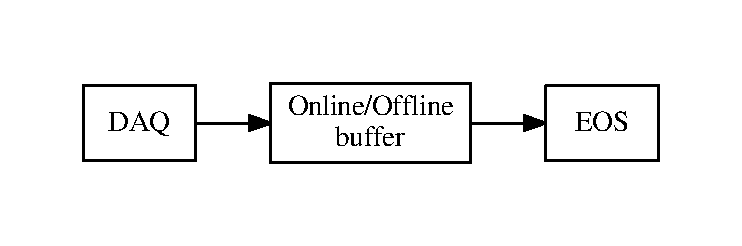
\includegraphics[height=1.5cm,clip,trim=0 10mm 0 10mm]{big-picture.pdf}
  \end{center}

  Recent \textbf{upward revision} of \textit{Data Scenarios Spreadsheet}:
  \begin{itemize}
  \item \href{http://docs.dunescience.org:8080/cgi-bin/ShowDocument?docid=1086}{DocDB 1086-v6} (let's put any and all updates here)
  \item[$\rightarrow$] 25-50Hz, 5ms, 6APA, 2-4$\times$ compression, 25-50M events.
  \end{itemize}
  Implications on \textbf{buffer requirements}
  \begin{itemize}
  \item 25-50TB buffer disk, 
  \item 30-60 parallel HDD writes, 
  \item 1.5-3.0 GByte/sec throughput.
  \end{itemize}
\end{frame}

\begin{frame}
  \frametitle{Data Scenario Implications on Buffer}

  Required to have \textbf{3 days buffer beam+cosmics}.

  \begin{center}
    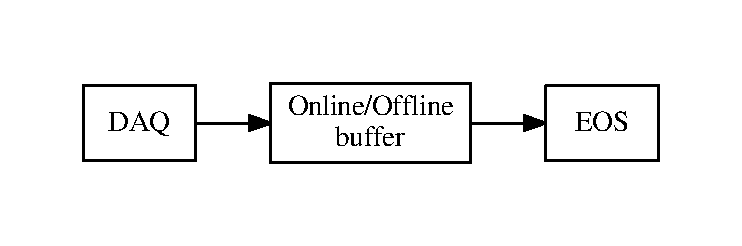
\includegraphics[height=1.5cm,clip,trim=0 10mm 0 10mm]{big-picture.pdf}
  \end{center}

  Recent \textbf{upward revision} of \textit{Data Scenarios Spreadsheet}:
  \begin{itemize}
  \item \href{http://docs.dunescience.org:8080/cgi-bin/ShowDocument?docid=1086}{DocDB 1086-v6} (let's put any and all updates here)
  \item[$\rightarrow$] 25-50Hz, 5ms, 6APA, 2-4$\times$ compression, 25-50M events.
  \end{itemize}
  Implications on \textbf{buffer requirements}
  \begin{itemize}
  \item 135-270TB buffer disk, 
  \item 30-60 parallel HDD writes, 
  \item 1.5-3.0 GByte/sec throughput.
  \end{itemize}
\end{frame}

\begin{frame}
  \frametitle{Back of the envelope estimate}
  
  If assume \textbf{1Gbps NICs}:
  \begin{itemize}
  \item \textbf{25 concurrent network streams}
  \item NIC is bottleneck so \textbf{minimum of 25 hosts} writing \textbf{2-3 disks}
  \item Beneficial side-effect: leaves plenty of idle CPUs to load up doing other, useful and prompt tasks.
  \end{itemize}

  If assume \textbf{10Gbps NICs}:
  \begin{itemize}
  \item \textbf{3 concurrent network streams}
  \item SATA is bottleneck so \textbf{minimum of 6 hosts} writing \textbf{10 disks}
  \item Hosts: fewer, bigger, more expensive, less ``off-the-shelf''.
  \item CPUs loaded just doing I/O, little room for other processing.
  \end{itemize}
  \vspace{5mm}

  A \textbf{quantitative investigation} based on assumptions of rates,
  bandwidths, processing times, etc is being developed with the
  \textbf{Ersatz Simulation} package. Links:
  \href{https://indico.fnal.gov/conferenceDisplay.py?confId=12498}{DAQ
    Sim presentation},
  \href{https://github.com/brettviren/ersatz}{GitHub}

\end{frame}

\begin{frame}
  \frametitle{Buffer Design - Two Options}
  
  \begin{description}
  \item[UOOB] Unified Online/Offline Buffer hosts
    \begin{itemize}
    \item[$\rightarrow$] Shared hosts, local disk for data hand-off.
    \end{itemize}
  \item[DOOB] Dedicated Online/Offline Buffer hosts
    \begin{itemize}
    \item[$\rightarrow$] Separate layers, network for data hand-off.
    \end{itemize}
  \end{description}

\end{frame}

\begin{frame}
  \frametitle{Unified Online/Offline Buffer}

  Online/offline interface: file-hierarchy on shared local disks.  

  \begin{columns}
    \begin{column}{0.4\textwidth}
      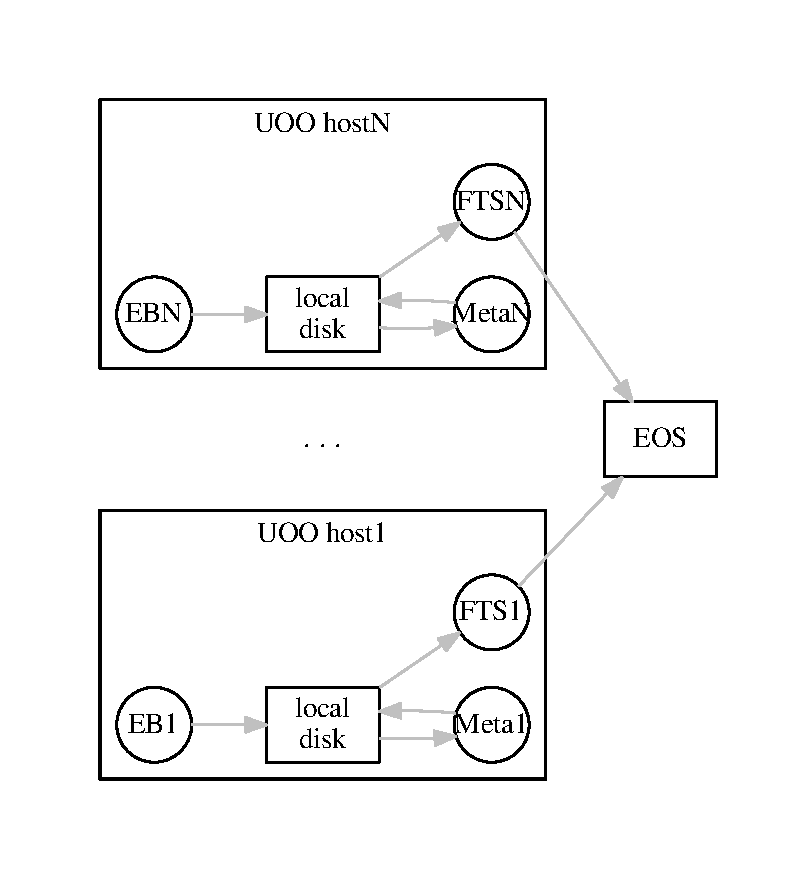
\includegraphics[width=\textwidth,clip,trim=5mm 0 5mm 0]{uoob-join.pdf}
    \end{column}
    \begin{column}{0.6\textwidth}
      Each UOOB computer must host:
      \begin{itemize}\footnotesize
      \item DAQ Event Builder node.
      \item File management glue scripts.
      \item File metadata producer.
      \item FTS instance.
      \item Logic to handle DAQ/FTS disk contention.
      \item Online/offline contract on detailed file locations.
      \end{itemize}
    \end{column}
  \end{columns}
\end{frame}

\begin{frame}
  \frametitle{Dedicated Online/Offline Buffer} 
  \begin{columns}
    \begin{column}{0.4\textwidth}
      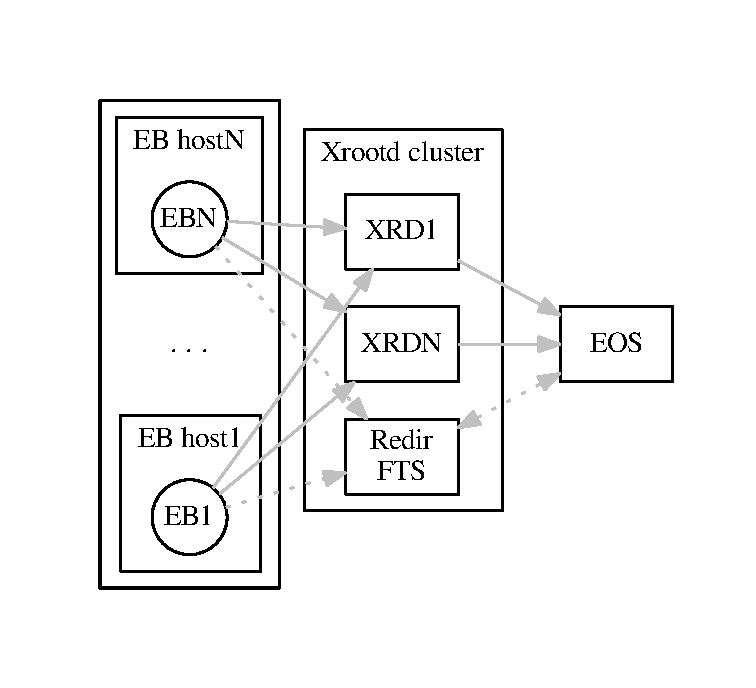
\includegraphics[width=\textwidth,clip,trim=5mm 0 5mm 0]{doob-join.pdf}
    \end{column}
    \begin{column}{0.65\textwidth}
      Dedicated ``layer'' in distributed graph
      \begin{itemize}\footnotesize
      \item Each EB needs to know only about XRD redirector.
      \item Transfers still load-balanced.
      \item Single FTS instance, share XRD redir host.
      \item Direct XRD transfer to EOS, governed by FTS.
      \item Decoupled Online and Buffer specs.
      \item XRD$_i$ nodes run metadata job after receive file.
      \item Interface specification = XRD URL namespace
      \end{itemize}
    \end{column}
  \end{columns}
  
\end{frame}


\begin{frame}
  \frametitle{Some pros/cons of each}

  UOOB:
  \begin{description}
  \item[pro] one less overall layer, file system hand-off maybe more
    familiar than XRD (?).
  \item[con] tight coupling in design and procurement, denser CPU
    requirement, O/O interface protocol more complex.  Multiple FTS
    (not big problem), FTS$\to$EOS mediated transfers.
  \end{description}

  DOOB:

  \begin{description}
  \item[pro] more distributed, leads to naturally more available CPU,
    decouples design and procurement, more fault-tolerant, O/O
    interface protocol simple.  Direct XRD$\to$EOS FTS-initiated
    transfers (EOS is native XRD).
  \item[con] requires extra layer, DAQ/EB needs XRD client lib (but not
    ROOT) or must use \texttt{xrdcp} unix command and thus its own
    local storage
  \end{description}
\end{frame}

\begin{frame}
  \frametitle{Take Away}
  \begin{itemize}
  \item We are looking to quantitatively understand the protoDUNE/SP
    online/offline needs.
  \item Likely major decision: 1Gbps vs. 10Gbps NICs
    \begin{itemize}
    \item[$\rightarrow$] want bottleneck at network or CPU/DISK?
    \end{itemize}
  \item Two design options exist:
    \begin{description}
    \item[uoob] concentrated complexity, tightly coupled, one less layer.
    \item[doob] simpler, more distributed but one extra layer, requires XRD.
    \end{description}
  \end{itemize}
  \textbf{What are our external constraints?  (how much \$\$\$?)}
\end{frame}

\end{document}


%%% Local Variables:
%%% mode: latex
%%% TeX-master: t
%%% End:

%%% Local Variables:
%%% mode: latex
%%% TeX-master: t
%%% End:
